This chapter presents necessary background to the individual topics used in this
thesis. In section\,\ref{sec:variability_modeling}, we recapitulate
basic concepts, notations, and terminology regarding variability modeling. In
section\,\ref{sec:evolving_solftware}, we outline different aspects of software evolution.
section~\ref{sec:assessing_performance} discusses the assessment and testing of
performance and finally, section\,\ref{sec:performance_prediction_models}
recalls methodology to predict performance behavior for configurable systems. In Section\,\ref{sec:relatedwork} we
review a body of related work that has either touched on topics similar to ours, or pursues a similar methodology, yet with different basic premises.

\section{Variability Modeling} \label{sec:variability_modeling}
The design and development of configurable software systems is conceptually
divided into \emph{problem space} and \emph{solution space} \citep{czarnecki_generative_2000}. The problem space
comprises the abstract design of features that are contained in the software
system as well as constraints defined among features, such as dependencies or mutual exclusion.
The solution space describes the technical realization of features and the
functionality described by and associated with features, e.g., implementation
and build mechanisms. That is, features cross both spaces since they are mapped
to corresponding code artifacts.

A common way to express features and constraints in the problem space is to
define a \emph{variability model}, or \emph{feature model}, which subsumes all
valid configurations
\citep{kang_feature-oriented_1990,thum_reasoning_2009,apel_feature-oriented_2013}.
There are different and equivalent syntactical approaches to define feature
models, for instance, a propositional formula $F$ over the set of features of
the configurable software systems \citep{batory_feature_2005}. In this case, a
configuration is valid with respect to the feature model if and only if $F$
holds for all selected features being true and all unselected features being
false, respectively.
However, a more practical and more commonly used way to express feature models
are graphical tree-like \emph{feature diagrams}
\citep{apel_feature-oriented_2013}. In a feature diagram, features are ordered
hierarchically, starting with a root feature and subsequent child features. By
definition, the selection of a child feature requires the parent feature to be
selected as well. Child features can either be labeled as \emph{optional}
features  or \emph{mandatory} features; the latter ones need to be selected in
every configuration.
Moreover, feature diagrams
provide a syntax for two different types of feature groups, \emph{or-groups} and
\emph{alternative-groups}. For an or-group, at least one of the group's features
needs to be selected for a valid configuration, whereas for an alternative-group
exactly one out of the group's mutually exclusive features must be selected. In
addition to the feature hierarchy, constraints, which cannot be expressed by
the tree-like structure, are referred to as \emph{cross-tree constraints}.
Cross-tree constraints, depending on the notation, are depicted by arrows
between two features or simply added to the feature diagram as a propositional
formula. For two features $f_1$ and $f_2$, a cross-tree constraint means
that for feature $f_1$ to be selected, either the selection of $f_2$ is
required/implied or excluded.

An introductory example for the syntax and semantics of feature diagrams is
provided in Figure~\ref{fig:introduction_fm}. In this example, an imaginary
vehicle propulsion can be configured with eight valid configurations. The
vehicle requires an engine, and therefore feature \textsf{Engine} is mandatory.
At least one out of the three features \textsf{Hybrid}, \textsf{Piston} and 
\textsf{Electric} needs to be selected. For a piston engine, we can select 
either the feature \textsf{Diesel} or \textsf{Petrol}. A petrol engine requires
additional ignition sparks in contrast to a Diesel engine. For an electric
engine, we require a battery, hence, the feature \textsf{Battery} is mandatory.
In addition, the feature model specifies two cross-tree constraints: First, the
feature \textsf{Tank} is optional, yet once a piston engine is selected, we
require  a tank. Second, if we want to use the \textsf{Hybrid} functionality
(e.g., use both electric and piston engine simultaneously), we require to have both a piston
and an electric engine.

\begin{figure}[htbp]
  \centering
  
  	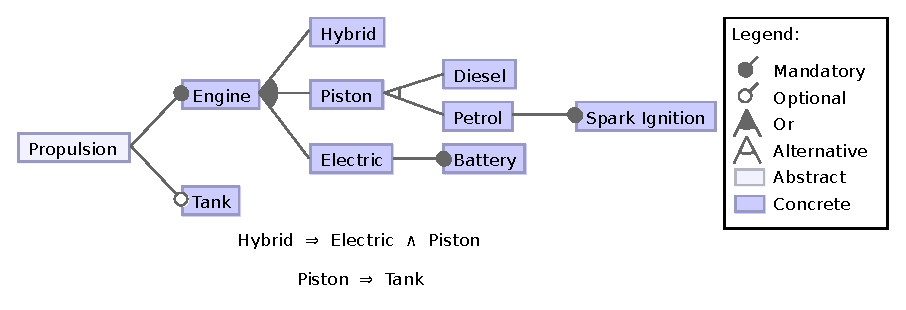
\includegraphics[width=0.85\textwidth]{images/introduction_fm.eps}
  \caption{Feature diagram for a feature model with eight valid configurations;
  two cross-tree constraints are specified as propositional formulas over
  features}
  \label{fig:introduction_fm}
\end{figure}

\section{Software Evolution} \label{sec:evolving_solftware}
The first notion of the software development process is usually
developer-centered and merely focuses on software being designed, implemented,
tested, and eventually being released and deployed.
Maintainability is a generally recognized software quality
property to look after, and maintenance is, of course, essential to every
successful software system \cite{liggesmeyer_software-qualitat:_2009}. Nonetheless, less attention is given to
the ability to adapt a software system to changing requirements (evolvability) rather than maintaining it to keep functionality
working \citep{parnas_software_1994}. Software evolution and evolvability, such
as software itself are manifold. Software evolves in many ways ranging from
maintenance (refactoring, bug-fixes, and patches) to adapting to changed
requirements (adding, removing, reorganizing functionality, and variability).
Modern software systems not only often ship with a variety of configuration
options to select from, they also employ routines to be build and sometimes even
make use of or are part of platforms, such as apps or plugins. That is,
software evolution affects all aforementioned aspects, maintainability as
well as evolvability can degrade as software evolves.

\subsection{Software Erosion}
The negative symptoms of software evolution which are referred to as
``architectural erosion'' \citep{breivold_systematic_2012} have
been addressed by many researchers.
Most of existing research so far though focuses on evolution with regard to
software architecture \citep{breivold_systematic_2012}. The main driving factors leading to symptoms of decay
identified by \cite{perry_software_1991} are architectural erosion and
architectural drift. While architectural drift subsumes developers'
insensitivity when not following a systems architecture or respective guidelines while making changes, architectural erosion subsumes ignoring and violating the existing software
architecture. \cite{parnas_software_1994} argues that as software evolves, software is maintained
and evolved by developers who are not necessarily familiar with the initial
architectural design. Therefore, knowledge about the architecture can become
unavailable as software evolves. Although the unfavorable effects of software
evolution do not break a system necessarily and imminently, the software becomes ``brittle'' \citep{perry_software_1991}
as maintainability as well as evolvability degrade. Concrete  symptoms of software
erosion on the implementation level have been documented. 

\cite{zhang_variability_2013} have studied erosion symptoms for a large-scale
industrial software product line with compile-time variability using
preprocessor directives.
The authors identify variability-related directives and clusters of those that
tend to become more complex as the software evolves. The negative effects, or symptoms of software
erosion are described as, but not limited to \emph{code replication} and
inter-dependencies between code elements, such as \emph{scattering} and
\emph{tangling}. Code scattering describes the phenomenon of code belonging to
a certain feature being scattered across multiple units of implementation,
such as modules, whereas code tangling means that code from different and
potentially unrelated features in entangled within a single module. A figurative
and recapitulative term to refer to the trade-off between postponed maintenance
or QA tasks and the corresponding cost is \emph{technical debt}
\cite{guo_tracking_2011}; the metaphor summarizes the growing risk of quality degradation for eroding software.

\cite{passos_feature_2015} have studied the extent of usage of scattering for device-drivers
in the Linux kernel. Despite scattering being quite prevalent, their
findings suggest that the kernel architecture is robust enough to have evolved
successfully. Nonetheless, platform drivers in the Linux kernel seem more
likely to be scattered than non-platform drivers. They conclude that this is a
trade-off between maintainability and performance: a more generalized and
abstract implementation for platform-drivers in this case could possibly avoid
scattering, yet refactorings in this manner did not seem to be necessary or
worth the effort yet. 


\subsection{Variability Evolution}
Apart from architecture evolution, the variability offered by software systems
evolves as well. For configurable software systems,
evolution steps will not only affect artifacts in the solution space, yet also
be visible in changes in the respective variability models in the problem space.
Although the variability aspect of software evolution has not gathered as
much attention as architecture in the past, more and more
research has emerged recently to address and understand variability evolution.

\cite{peng_analyzing_2011} proposed a classification of variability evolution patterns that
conceives evolution as adaption to changing (non-)functional requirements and
contexts. For a context in that sense, two categories exist. A driving context
determines, whether a variability model and respective variants can meet
functional requirements in the first place. A supporting context by definition
determines how non-functional properties are strengthened or weakened. 
Any changed requirement is likely to change the contexts for a software systems
variability model and, therefore, will make adaptations of the variability
model necessary. Within their classification method, \cite{peng_analyzing_2011} identify major
causes for variability evolution, comprising (a) new driving contexts emerging,
(b) weakened supporting contexts (for instance, due to new non-functional 
requirements), and (c) unfavorable trade-offs for non-functional properties.

To understand single evolutionary steps, several catalogs of variability
evolution patterns have been proposed. \cite{peng_analyzing_2011} present three patterns,
where either a new feature is added, a mandatory feature becomes optional, or a
mandatory/optional feature is split into alternative features. \cite{seidl_co-evolution_2012} suggest a catalog of
patterns for co-evolution of variability models and feature mappings that additionally introduces code clones, splitting a feature
into more fine-grained sub-features, and feature removal as evolution patterns.
In addition, \cite{passos_towards_2012} have studied variability evolution in
the Linux kernel and present a catalog of patterns where features are removed from the
variability model, but remain a part of the implementation. Their
catalog, among others, includes feature merges, either implicit (optional feature merged
with its parent) or explicit.

The classification proposed by \cite{peng_analyzing_2011} is a general and formalized approach
that, as well as \cite{seidl_co-evolution_2012} and \cite{passos_towards_2012}, describes
elementary evolution patterns which can be composed to more complex patterns. Nonetheless, no
comprehensive catalog of variability evolution patterns so far has been
proposed.

\section{Assessing Performance} \label{sec:assessing_performance}
While the last three sections covered software evolution and variability
modeling, we now step forward to the topic of software performance. This
section will outline the term performance with respect to software systems as
well as to possible measurements. We provide a brief look at the general performance
testing setup and the required prerequisites, including suitable benchmarks.
Finally, we provide the statistical background to summarize, interpret and
compare performance measurements accurately.

\subsection{What is Performance?}
The performance of software systems is, like software quality, primarily a
matter of perspective. While an end user might consider practical aspects to be
more important, from a developer’s perspective, performance relates to and is
best described by non-functional properties
\citep{liggesmeyer_software-qualitat:_2009,molyneaux_art_2014}.
While functional properties subsume what exactly a software system does, non-functional
properties describe how (good or bad) a software system is at providing the
functionality offered \citep{liggesmeyer_software-qualitat:_2009}. The notion
of good and bad in this sense corresponds to non-functional requirements (NFR),
that is, software with ``good'' performance behavior does not violate its NFRs.
The categories of NFRs that shape performance behavior are manifold. According to \cite{molyneaux_art_2014}, the categories or
\emph{key performance indicators} (KPIs) include 

\begin{itemize}
  \item availability
  \item response time,
  \item throughput,
  \item resource utilization, and in a broader scope also 
  \item capacity.
\end{itemize}

Time-related KPIs are availability and response time, whereby
availability describes the time or time ratio that the software is available to
the end user, and response time subsumes the time it takes to finish a request
or operation. Throughput as a category subsumes the program behavior with
respect to program load, such as hits per second for a Web application or
amount of data processed per second. Resource utilization describes the extent
to which a software system uses the physical resources (CPU time, memory, and
disk, or cache space) of the host machine. Finally, from a Web-centered
perspective, capacity describes measurements with respect to servers and
networks, such as network utilization  (traffic, transmission rate) and server
utilization, such as resource limitations per application on a host server
\citep{molyneaux_art_2014}.

Consequently, the assessment of performance requires a context or testing
target that corresponds to the assessed system under test (SUT). For instance,
for a simple command-line compression tool, suitable KPIs are response time and
throughput, whereas performance for an online shop Web application is better
outlined by availability and capacity.

\subsection{Performance Testing}
The first step in performance testing, prior to defining relevant KPIs and
metrics, is to specify a system operation or \emph{use case}
\citep{woodside_future_2007} to assess performance for. A typical use case includes a well defined task or
workload to process, expected behavior, outcome, and performance
requirements as previously discussed. For the SUT, however, we require a
version that does compile or, in case it is interpreted, is syntactically
correct \citep{molyneaux_art_2014}. With regard to performance assessments as part of
the development process, a code freeze should be obtained since measurement
results are likely to become meaningless for later versions. In addition to
that,  the machine or setup used for performance measurement should ideally be
as close to the production environment as possible, but at least be documented
to compare different runs \citep{molyneaux_art_2014}.

Finally, one or more benchmarks need to be selected to simulate  the program
load for the respective use case. A benchmark, all in all, needs to be
representative, i.e., should relate to the use case or requirement one
 wants to validate. While benchmarks for file compression usually include
multiple different types of media data (text, sound, pictures) such as the
Canterbury corpus\footnote{The Canterbury corpus can be found
here, \url{http://corpus.canterbury.ac.nz/}.}, Web applications can be exposed
to handling with a number of simulated users at the same time
\citep{molyneaux_art_2014}. Benchmarks have often been standardized within
research and engineering communities to provide comparable performance
measurements. A popular example is the Software Performance Evaluation
Corporation (SPEC), a consortium providing a variety of benchmarks such as the
CPU2000\footnote{The benchmark description can be found at \url{https://www.spec.org/cpu2000/}.} processor benchmark consisting of programs with both floating point and integer operations.
Moreover, benchmarks, in a sense of repeatable program load, can be obtained
from load generation software such as ApacheBench\footnote{Manual page of the
Apache tool \texttt{ab}, \url{http://httpd.apache.org/docs/2.4/en/programs/ab.html}.}
for the Apache Web server or simply by measuring performance for test cases
\citep{heger_automated_2013,nguyen_industrial_2014}.

Performance testing heavily relies on tool support, especially for repeating
test cases and recording measurements. Since the
tool solutions for performance testing vary from domain, scale, and purpose, we
will outline  only the general tool architecture. \cite{molyneaux_art_2014}
describes four primary components for a performance testing setup: a scripting module, a
test management module, a load injector, and an analysis module. A scripting module handles the generation or
repetition of use cases which, for instance, can be recorded prior to the test
for Web applications. A test management module creates and executes a test
session, whose program load is generated by one or more load injectors. A load
injector can provide a benchmark by generating items to process, or can simulate
a number of clients for a server-side application. An analysis module, finally,
collects and summarizes data related to the performance testing target. We present more on
summarizing and comparing recorded results in the
sections\,\ref{sec:statistical_considerations} and~\ref{sec:summarization}.


\section{Performance Prediction
Models}\label{sec:performance_prediction_models} In the previous section, we referred to performance, or in detail, the KPIs, as
possible testing targets, which we validate against non-functional requirements.
However, in a broader sense, software performance has become an aspect of
software engineering referred to as \emph{software performance engineering}
(SPE) \citep{woodside_future_2007}.
A lot of effort has been spent to study and describe performance behavior as well
as to improve performance quality. Besides the analysis of concerns or
requirements with respect to performance, SPE comprises performance testing as
well as performance prediction \citep{woodside_future_2007}. Performance
prediction aims at modeling and estimating performance behavior for different
use cases or configurations. The first approaches to performance prediction
models describe the underlying software system component or operation from which
performance estimations are then deduced. These so-called \emph{model-based prediction models} enable a performance estimation early in the development process since no actual
performance measurement is required \citep{woodside_future_2007}. In contrast
to model-based approaches, measurement-based approaches have emerged. These \emph{measurement-based prediction models} are based on a sample of performance
measures which are used to learn a software system's performance behavior
\citep{woodside_future_2007}. More recently, measurement-based prediction models that emphasize variability have been
proposed, of which we will discuss three approaches in the remainder of
this section.

\paragraph{Learning Performance} In essence, learning and predicting
performance behavior for a configurable system means nothing different than finding an
approximation $\hat{f}$ for a function $f: C \rightarrow \mathbb{R}$ where $C$
is the set of configurations and $f(c) \in \mathbb{R}$ with $c \in C$ is the corresponding performance measurement. The
accuracy of the approximation $\hat{f}$ describes how the estimated performance
$\hat{f}(c)$ deviates from the actually measured performance $f(c)$. 
Different approaches to construct such an approximation, referred to as a
\emph{performance prediction model}, emerged recently. All approaches utilize
two samples of configurations and corresponding performance
measurements to build and validate the model. A training sample is used to
learn the approximation from, whereas a testing sample is used to assess the
prediction error rate of the previously learned approximation. 
%While the
%approaches mentioned below differ in the expression of a performance prediction
%model, all require ``meaningful'' training samples and stress the importance of
%sampling strategies.

A straightforward methodology to learn performance behavior was proposed by
\citep{guo_variability-aware_2013}.
The authors utilize classification-and-regression-trees (CART), akin to decision trees, to derive a top-down classification hierarchy for a
given sample. The approach supports progressive (and random) sampling, i.e.,
the performance model is constructed several times while the size of the
training sample is successively increased. The CART is constructed by
recursively partitioning the sample into smaller segments which best describe a
class. It is worth mentioning that the estimation using CART is not limited to
binary configuration options, but supports numeric features as well. Moreover,
the approach by \citep{guo_variability-aware_2013} does not produce any further
computation overhead besides the measurement effort and the construction of a CART.

A different approach to modeling performance behavior was
proposed by \cite{zhang_performance_2015}. The authors propose an approach to construct
performance prediction models based on a Fourier description of the
performance-describing function $f$, which maps each configuration to a
corresponding performance measurement. The principal idea is to approximate a
Fourier series approximating the function  $f$, and
learning all coefficients of the Forier series terms.

The number of terms is exponential in the number of configuration options. The main
characteristic of this approach is that, prior to learning a performance
prediction model, a desired level of prediction accuracy can be specified. That
is, the approach automatically chooses the sample size required to learn the
prediction model accordingly.

A third approach to model and predict performance behavior,
\emph{SPLConqueror}, was proposed by \cite{siegmund_predicting_2012}. The
authors describe performance behavior  for a configuration as the accumulated influence of
features, from which the configuration is composed, and respective feature
interactions. To estimate the influence of single features and feature
interactions, the authors propose a number of sampling strategies. Single
features are assessed by comparing the performance of two different
configurations per feature: For a feature $f$, two valid configurations are
compared, whereby both configurations have the minimal number of features
selected that are not excluded by the selection of $f$. While for one
configuration $f$ is selected, it is deselected for the other one. The
difference between the performance measures for both configurations is the estimate
$\Delta_{min(f)}$ for the performance influence of feature $f$. Feature
interactions that are performance-relevant are detected automatically in a similar manner. The
main idea is, that a feature $f$ is more likely to interact with other features,
the more features are selected along with $f$. Therefore, if $f$ interacts, the
influence of feature $f$,  $\Delta_{min(f)}$ differs from the influence of $f$,
when estimated using configurations where the maximal number of features selectable
together with $f$ are used. Based on the set of interacting features, three
heuristics are employed to detect feature interactions. Simple feature
interactions are detected using pair-wise sampling
\citep{siegmund_predicting_2012,apel_feature-oriented_2013}, whereas
higher-order feature interactions are often composed from simpler ones, or centered
around a small subset of hot-spot features \citep{siegmund_predicting_2012}.
Finally, for an arbitrary configuration, the performance can be predicted by the
sum of influence estimations per feature and feature interaction.

The idea of predicting performance by estimating the influence of feature
and feature interactions was further developed by \cite{siegmund_performance-influence_2015} by
proposing performance-influence models for both binary and numeric
configuration options. A performance influence, similar to \emph{SPLConqueror},
predicts performance by computing the sum of previously learned influence
estimates. The novelty of this approach lies in the way the terms describing
the influence of feature and feature interactions are learned and not
derived from a sampling strategy.
Instead of a single constant performance influence estimate, each term can contain of a
number of functions, such as linear, quadratic, or logarithm functions, or
compositions thereof. This does not only allow the developer to incorporate
domain knowledge by preselecting functions. Moreover, but also by introducing
combinations of non-linear functions and learning the coefficients using linear
regressions, it enables learning a non-linear function. The algorithm commences
with the selection of terms and successively extends and reduces the term selection to increase 
the prediction accuracy. The outcome, similar to
\cite{siegmund_predicting_2012}, is a linear function whose terms represent the estimated influence of features and
feature interactions on performance.

All aforementioned approaches rely on performance measurements and, to
some extent, also on a  sampling strategy. While the approaches by
\cite{siegmund_predicting_2012,siegmund_performance-influence_2015} essentially describe sampling strategies,
the approach proposed by \cite{zhang_performance_2015} is able to work with random samples, and the
approach of \cite{guo_variability-aware_2013} allows a smaller sample to be
extended progressively \citep{guo_variability-aware_2013}.
As performance measurements entails an expensive and time-consuming process,
\cite{sarkar_cost-efficient_2015} have investigated different sampling
strategies in this domain.
The authors compare progressive sampling, where sample sizes are increased
successively until the learned prediction model performs accurately enough, and projective
sampling, where the optimal sample size is estimated based on the expected
learning curve, with respect to cost and prediction accuracy. They advocate the
use of projective sampling over progressive sampling. In addition, the authors
propose and evaluate an own sampling heuristic to select an initial sample for
progressive sampling. This sampling heuristic is based on feature frequencies
and outperforms t-wise sampling, such as pair-wise sampling
\citep{sarkar_cost-efficient_2015}.

\section{Related Work}\label{sec:relatedwork}
While to the best of our knowledge, there exists no previous work on
exhaustively presenting a methodology to understand and comprehend performance
evolution of configurable software system, there is a body of work that has
either touched on similar topics, or pursues a similar methodology, yet with
different basic premises. In the following, we present and summarize related
work to emphasize thelimited scope of our work, and to give an outline of
possible future research directions. Further note that we describe here only
additional approaches to the ones we have already discussed in the previous
sections.

\paragraph{Visualization of Software Evolution.}
Throughout our methodology, we have frequently used diverse visualizations of
data obtained from repository mining, for instance, for commit activity, and as
a basis for revision sampling strategies. In addition, we have taken into
account similar data in the interpretation of our performance evolution history
data in section. Therefore, as software evolves it is inevitable to not
consider those data to obtain more complete and integrated insights.
Aggregation and visualization of aforementioned data records can help to sketch
and understand possible coherences.

\cite{german_visualizing_2006} have presented a comprehensive tool,
\emph{softChange}, to visualize multiple aspects of a software system’s
evolution history, including commit and file activity graphs, authorship
overviews, and visualizations of file coupling. While their tool is not
designed with regard to a specific research direction, the authors stress the
importance of means to aggregate and analyze software trails in order to
explore and understand software evolution. Joint visualizations
of software trails as well as performance evolution history data is a promising
augmentation in the comprehension of multi-layered software evolution.

\cite{wu_exploring_2004} have presented presented an integrated approach to
visualize multiple different measurements over time. Their proposed
\emph{evolution spectrum graphs} are inspired by spectrum visualizations for
audio signals. A spectrum in their context can, for instance,  be a list of files, for which
different measurements are illustrated over time. While this approach allows
for a global overview over an arbitrary timespan, it also can sketch
fine-grained changes and trends over time. Although, according to the authors, the
visualizations need to be tailored to the target system with respect to
coloring and spectrum selection, evolution spectrum graphs can be a useful
means to aggregate and visualize various single-valued measurements for a
spectrum of variants for configurable software systems.

To conclude with a broader overview on visualization tools for further reading,
\cite{storey_use_2005} have surveyed twelve tools (including the previously
mentioned two) that intend to visualize any kind of human activities in
software development with a string focus on software evolution. The authors
evaluate the different tools with respect to different aspects, including
intent of the tools, the information sources utilized by the tools, the form of
presentation offered by the tools, and the effectiveness in terms of
feasibility and validity.

We see these lines of work orthogonal to our methodology such that we can
incorporate different visualization techniques when it comes to evaluating and
understanding the performance evolution of configurable software systems.

\paragraph{Power Consumption Evolution}
\cite{hindle_green_2015} have proposed a methodology, \emph{green mining}, to
measure and model the evolution of power consumption across different versions of a
software system. Using their methodology, the authors have documented the power
consumption evolution history of two different software systems, and identified
feasible metrics to summarize power consumption. 

Compared to our proposed methodology, green mining considers only 
one-dimensional evolution of power consumption as different software variants
are not taken into account, yet green mining examines the relationship between
power consumption and further quality attributes. That is, we believe that
interpreting performance evolution results in an extended context of software
metrics with respect to software architecture, power consumption, and along
established software analyses should direct further research activities towards
a better understanding of software evolution.